
\part[Subalgoritmos]
{Funções}


\chapter[Subalgoritmos]
{Funções}



\section{Resumo}

Uma função é um conjunto de instruções que, ao final da função, executa uma tarefa. Todo programa C possui pelo menos uma função, a \emph{main}.

%\begin{chapreferences}{1.}
%\bibliography{playcb}
%\bibliographystyle{plain}
%\nocite{cbook}
%\nocite{sb6}
%\nocite{glfw}
%\nocite{cppbook}

%\end{chapreferences}

% \begin{chapreferences}{1}

% \bibitem{sb6}
% {\em OpenGL SuperBible}.
% \newblock Pearson Education Inc, 6 edition, 2014.

% \bibitem{glfw}
% Marcus Geelnard and Camilla Berglund.
% \newblock {\em GLFW - Reference guide}, 2010.
% \newblock API version 2.7.

% \bibitem{cbook}
% Brian~W. Kernighan and Dennis~M. Ritchie.
% \newblock {\em The C Programming Language}.
% \newblock 1989.

% \bibitem{cppbook}
% Stanley~B. Lippman, Josés Lajoile, and Barbara Moo.
% \newblock {\em C++ Primer}.
% \newblock 2013.
% \end{chapreferences}

\begin{problems}
\prob
Crie o jogo Snake com as seguintes configurações
\begin{itemize}
\item
A cabeça não pode estar na mesma posição que o corpo
\item
A cabeça não pode estar na mesma posição que a parede
\end{itemize}
\emph{SUGESTÃO: Utilize a lógica do exercício \ref{ex:cap02_ex1} }

\label{ex:cap03_ex1}
\end{problems}

\section{Soluções}

\subsection{\ref{ex:cap03_ex1}Snake}
\begin{figure}[ht]
  \centerline{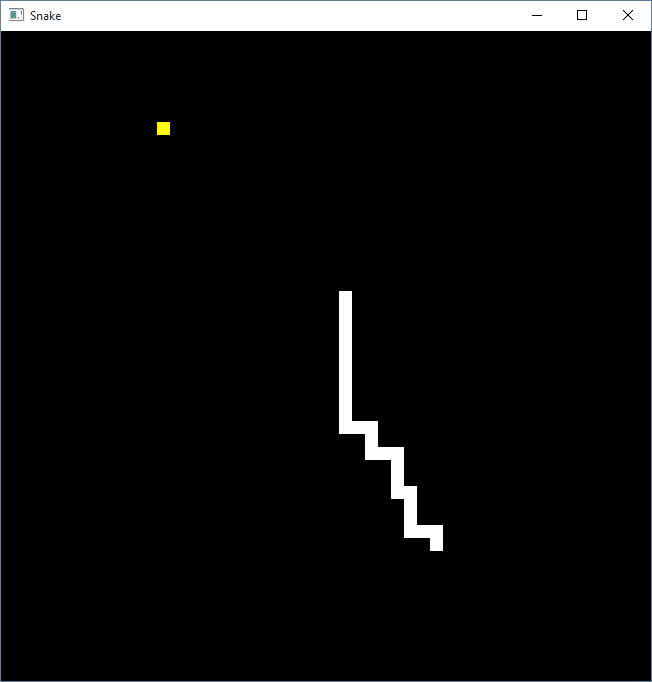
\includegraphics[width=.5\textwidth]{img/cap3_ex10.png}}
  \caption{Jogo Snake}
  \label{fig:cap03_ex1}
\end{figure}
Esta prática ilustra como a função \emph{ApertaTecla} e \emph{MudaLimitesJanela} podem ser utilizadas: a primeira para lidar com input de teclado \footnote{\url{http://pt-br.playcb.wikia.com/wiki/Aperta_Tecla}} e a segunda para ajustar o plano onde as geometrias serão desenhadas.
\lstinputlisting[caption=Código fonte de Snake, style=customc, label=lst:cap3_ex1]{src/ex10_snake.cpp}
